\documentclass{article}
\usepackage[italian]{babel}
\usepackage{listings}
\usepackage[letterpaper,top=2cm,bottom=2cm,left=3cm,right=3cm,marginparwidth=1.75cm]{geometry}

\usepackage{graphicx} % Required for inserting images

\title{
\textbf{Università degli studi di Napoli Parthenope\\
Laboratorio di Reti di Calcolatori\\
Progetto: \textbf{Università}}
}

\author {Davide Aiello 0124002594}

\date{}

\begin{document}



\begin{figure}[htp]
    \centering
    
\includegraphics[width=0.5\linewidth]{logo_uni.png}
    \maketitle
\end{figure}
\newpage
\section{Descrizione}


L'applicazione client/server parallelo per gestire gli esami universitari si propone di automatizzare e semplificare il processo di prenotazione e gestione degli esami. La segreteria, come interfaccia principale, inserisce dettagli sugli esami nel server dell'università, consentendo di salvare i dati su file. Inoltre, gestisce le richieste di prenotazione degli studenti, inoltrando tali richieste al server universitario.\\

Gli studenti possono interrogare la segreteria per verificare la disponibilità di esami per un determinato corso e inviare richieste di prenotazione. Il server universitario riceve le nuove informazioni sugli esami e le prenotazioni degli studenti, assegnando a ciascuna richiesta un numero progressivo. Questo numero viene inviato alla segreteria dal server universitario e successivamente trasmesso agli studenti, garantendo un tracciamento sistematico delle prenotazioni.\\

La struttura parallela del sistema consente una gestione efficiente e concorrente delle richieste, migliorando la scalabilità e la reattività del sistema. L'utilizzo di un server centrale favorisce la coerenza dei dati e semplifica la manutenzione. Complessivamente, il progetto mira a ottimizzare il processo di gestione degli esami universitari, garantendo un accesso agevole alle informazioni e una registrazione accurata delle prenotazioni degli studenti.

\section{Descrizione e schema dell'architettura}
\begin{figure}[htp]
    \centering
    
\includegraphics[width=1\linewidth]{architettura-rete.png}
    \caption{Architettura della rete}
\end{figure}

Richiesta esami:
\begin{itemize}
    \item Studente si connette a Segreteria e chiede se ci siano esami disponibili per un corso
    \item La segreteria riceve il nome del corso e lo inoltra al Server Universitario
    \item Il Server Universitario riceve il nome del corso e controlla se ci siano esami disponibili per il corso ricevuto
    \item Il Server inoltra la lista degli esami disponibili alla segreteria
    \item La Segreteria inoltra la lista degli esami disponibili allo studente che ha effettuato la richiesta
\end{itemize}

Aggiunta esami:
\begin{itemize}
    \item Segreteria inoltra al sever il nome del corso, la data di esame e il numero di CFU dell'esame da aggiungere.
    \item Il Server Universitario riceve la richiesta e salva sul file 'examsList' l'esame.
\end{itemize}

Prenotazione esame:
\begin{itemize}
    \item Una volta ricevuta dalla Segreteria la lista degli esami disponibili per il corso richiesto lo studente può decidere a quale prenotarsi inserendo il codice dell'esame e la sua matricola
    \item Lo studente inoltra alla Segreteria l'esame scelto e la marticola
    \item La Segreteria riceve l'esame e la matricola dello studente e l'inoltra al Server Universitario
    \item Il Server Universitario riceve esame e matricola e salva la prenotazione sul file di prenotazione dell'esame scelto associando a quest'ultima un Id univoco di prenotazione
    \item Il Server Universitario inoltra alla Segreteria il numero di prenotazione

\end{itemize}
\section{Dettagli implementativi dei client/server}
Il client scrive sul socket di connessione alla segreteria la struct Request che contiene:
\begin{itemize}
    \item requestType: tipo di richiesta effettuata
    \begin{itemize}
        \item requestType = 1: indica che lo studente richiede la lista delgi esami disponibili
    \end{itemize}
    \item Exam: struct Exam che contiente:
    \begin{itemize}
        \item name: nome del corso
        \item data: data del corso
        \item cfu: CFU del corso
    \end{itemize}

\end{itemize}

\begin{figure}[htp]
    \centering
    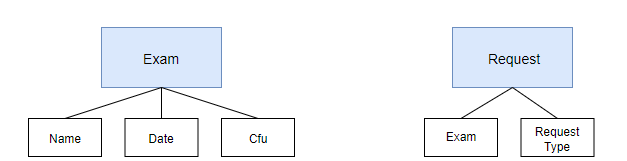
\includegraphics[width=1\linewidth]{struct.png}
    \caption{Dati inviati alla segreteria da parte dello studente}
    \label{fig:enter-label}
\end{figure}
\begin{lstlisting}[language=C]
struct Exam {
    char name[40];
    char date[25];
    short cfu;
};

struct Request {
    short requestType;
    struct Exam exam;
};
\end{lstlisting}
Lo studente inserisce il nome del corso che viene poi salvato nella struct availableExamRequest.exam.name.
Il campo requestType viene settato a 1.\\
Dopodichè viene creato il socket 'socketFD' e si effettua la connessione alla Segreteria.\\
Si scrive la struct availableExamRequest sul socket inviando così la richiesta alla segreteria.\\
La segreteria effettua una read sul socket connFD, se requestType == 1 allora si collega al server universitario, salva sulla struct retriveAvailableExamRequest l'esame ricevuto dallo studente e setta requestType a 2.\\
Esegue una write sul socket di connessione con il server universitario della struct e quindi invia al server la richiesta.\\
Il server esegue una read sul socket connFD, se requestType == 2, allora apre il file 'examList' e controlla quali esami salvati corrispondono al corso richiesto, salvando ogni esame disponibile su un array di struct Exam.\\
Successivamente scrive sul socket di connessione con la segreteria l'intero array con gli esami disponibili.
La segreteria riceve l'array di struct e lo inoltra allo studente che ha effettuato la richiesta che può ora visualizzare le date di esame per il corso richiesto.\\\\
Dopo aver ricevuto la lista degli esami disponibili per il corso richiesto, lo studente inserisce il codice dell'esame a cui desidera iscriversi e la propria matricola.
Codice e matricola vengono scritti sul socket di connessione con la segreteria socketFD, la segreteria riceve ed inoltra al server universitario quest'ultimi.\\
Il Server riceve il codice dell'esame e apre il file di prenotazioni che corrisponde all'esame richiesto ed aggiunge in coda al file la prenotazione dell'esame con il numero assegnatogli e la matricola.\\

\newpage
\section{Parti rilevanti del codice}
Richiesta da parte dello studetente della lista esami disponibili per un determinato corso:
\begin{figure}[htp]
    \centering
    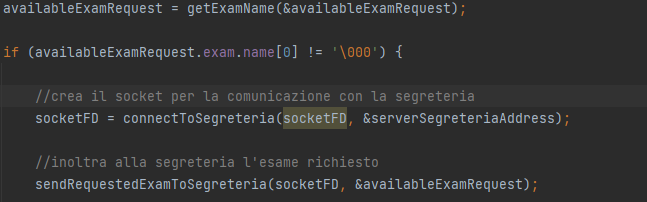
\includegraphics[width=1\linewidth]{richiesta esami disponibili.png}
\end{figure}
\\La Segreteria invia la server la richiesta ricevuta dallo studente:
\begin{figure}[htp]
    \centering
    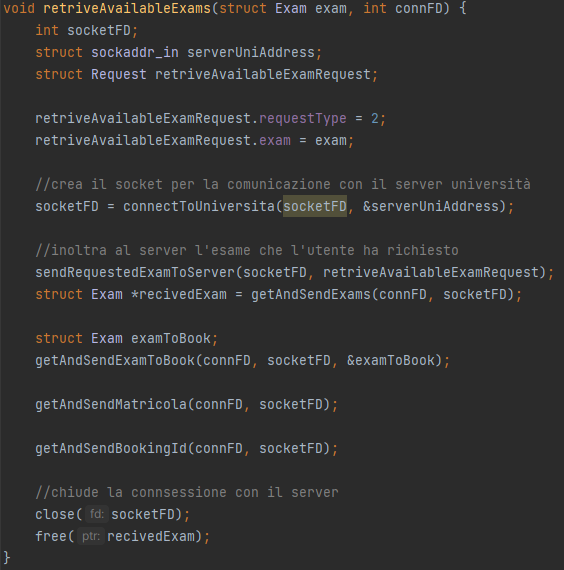
\includegraphics[width=0.8\linewidth]{retriveAvailableExamsSegreteria.png}
\end{figure}
\newpage
Il server Universitario invia alla Segreteria la lista degli esami disponibili per il corso richiesto:
\begin{figure}[htp]
    \centering
    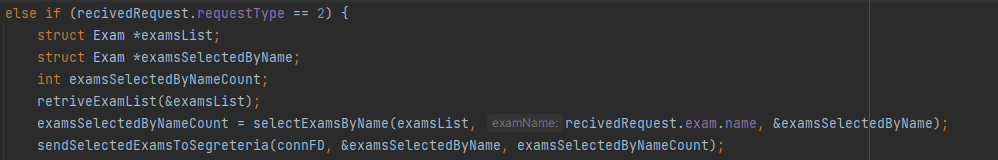
\includegraphics[width=1\linewidth]{retriveExamsListUnipng.png}
\end{figure}
\\La segreteria invia al server un nuovo esame da aggiungere:
\begin{figure}[htp]
    \centering
    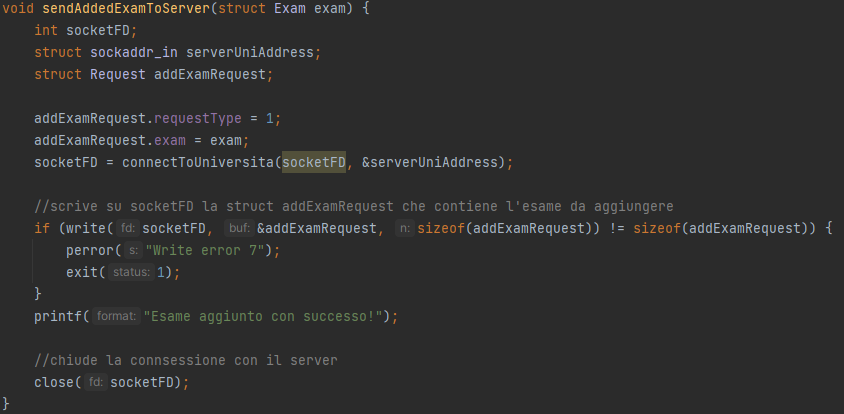
\includegraphics[width=1\linewidth]{addExamSeg.png}
\end{figure}
\\Il server aggiunge l'esame ricevuto sul file "ExamList":
\begin{figure}[htp]
    \centering
    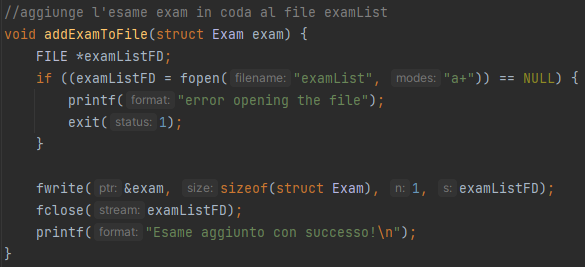
\includegraphics[width=0.8\linewidth]{addExamUni.png}
\end{figure}
\newpage
\section{Manuale}
\subsection{Istruzioni di compilazione:}
in progetto-universita/Wrapper:
\begin{itemize}
    \item gcc -c -o wrapper.o wrapper.c
\end{itemize}
in progetto-universita/universita:
\begin{itemize}
    \item gcc -c -o universita.o -I../Wrapper universita.c
    \item gcc -o Universita universita.o ../Wrapper/wrapper.o
\end{itemize}
in progetto-universita/segreteria:
\begin{itemize}
    \item gcc -c -o segreteria.o -I../Wrapper segreteria.c
    \item gcc -o Segreteria segreteria.o ../Wrapper/wrapper.o
\end{itemize}
in progetto-universita/studente:
\begin{itemize}
    \item gcc -c -o studente.o -I../Wrapper studente.c
    \item gcc -o Studente studente.o ../Wrapper/wrapper.o
\end{itemize}
\subsection{Istruzioni di esecuzione:}
in progetto-universita/universita:
\begin{itemize}
    \item ./Universita
\end{itemize}
in progetto-universita/segreteria:
\begin{itemize}
    \item ./Segreteria
\end{itemize}
in progetto-universita/studente:
\begin{itemize}
    \item ./Studente
\end{itemize}

\end{document}
